\subsection{Ordnungsrelationen}\index{Ordnungsrelationen}



\begin{bbwFillInTabular}{c|l}
  $a=b$                        & Gleichheit\noTRAINER{\hspace{20mm}}\\
  $\pi\ne 3$                   & \TNDF{Ungleichheit}\\
  $a<b$                        & \TNDF{$a$ ist kleiner als $b$}\\
  $3>1$                        & \TNDF{Analog:  ... ist größer als ...}\\
  $a\leq b$                    & \TNDF{$a$ kleiner als oder gleich $b$ }\\
  $a\geq 4$                    & \TNDF{Analog: $a$ ist gleich 4 oder größer als 4}\\
  $\pi\approx \frac{355}{113}$ & \TNDF{ungefähr gleich}\\
  $1 \ll 6.022 \cdot{} 10^{23}$ & ... sehr viel kleiner als...\\
  $10^{100} \gg 1000$           & ... sehr viel größer als...\\
  \hline
\end{bbwFillInTabular}


\subsection*{Aufgaben}

\GESO{\olatLinkArbeitsblatt{Ordnungsrelationen
    [A1ordn]}{https://olat.bms-w.ch/auth/RepositoryEntry/6029794/CourseNode/106261509036700}{1.,
    2. und 3. (ohne Aufgabe 4. und 5.)}}%% END olatLinkArbeitsblatt
\TALS{\olatLinkArbeitsblatt{Ordnungsrelationen [A1ordn]}{https://olat.bms-w.ch/auth/RepositoryEntry/6029786/CourseNode/106261509170117}{1., 2. und 3.}}%% END olatLinkArbeitsblatt
\GESO{\olatLinkGESOKompendium{1.2}{6}{2}}
\TRAINER{Keine Intervallschreibweise bei GESO}
%% %%%%%%%%%%%%%%%%%%%%%%%%%%%%%%%%%%%%%%%%%%%%%%%%%%%%%%%%%%%%%%%%%%%%%%%%%%%%%%%%%%%%%
\TALS{%% Intervall Notation nur bei TALS}

  \newpage
\subsubsection{Intervall-Notation}

%%\renewcommand{\arraystretch}3
\begin{bbwFillInTabular}{c|c|c}

  Relation & Zahlengerade & Intervallschreibweise \\
  \hline
  $a \geq 4$  &
  \TRAINER{\raisebox{-5mm}{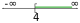
\includegraphics[width=40mm]{allg/alg/img/intervallGE4.png}}}
  \noTRAINER{\hspace{6cm}} & $[4;  \infty [$\\
      \hline
      
  $x\leq 5$ und $x > -2$  &
      \TRAINER{\raisebox{-5mm}{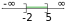
\includegraphics[width=40mm]{allg/alg/img/intervallM2T5.png}}}
      & \TNDF{$]-2; 5]$}\\
  
  \hline
  $-42 > z$  &
  \TRAINER{\raisebox{-5mm}{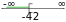
\includegraphics[width=40mm]{allg/alg/img/intervallLE-42.png}}} & \TNDF{$] -\infty ; -42[ $}\\
\hline  
\end{bbwFillInTabular}
%%\renewcommand{\arraystretch}1

\TALS{\subsection*{Aufgaben}

%%\GESO{\olatLinkArbeitsblatt{Ordnungsrelationen [A1ordn]}{https://olat.bms-w.ch/auth/RepositoryEntry/6029794/CourseNode/106261509036700}{4. und 5.}}%% END olatLinkArbeitsblatt
\olatLinkArbeitsblatt{Ordnungsrelationen [A1ordn]}{https://olat.bms-w.ch/auth/RepositoryEntry/6029786/CourseNode/106261509170117}{4. und 5.}}%% END olatLinkArbeitsblatt

}%% END TALS

\TNTeop{}
%% \newpage %% implicit
%%\GESOAadBMTA{22f}{10. b) 11. a) b) c) d)}
%%\TALSAadBMTA{13}{13.}
%%\TRAINER{Spätestens hier auf die Musterlösungswege im OLAT hinweisen.}
